\chapter{Carbohydrates: Fuel, Materials, and Identity Tags}

\begin{kaichang}
Gather four things: a sugar cube, a spoonful of cooked white rice, a tissue (or a small wad of cotton), and the line on a medical report showing your blood type---for example, ``A'' or ``O.''

Now guess: what common ``raw material'' connects these four things? Sugar cubes and rice are edible, but tissues are not; blood type cannot even be seen or touched and requires a blood sample to determine. What makes them one family?

Write down your guess. By this chapter's end, you will discover that their main components are actually \textbf{the same small molecule}---glucose. Only the assembly differs: the kind of chain, the angle of the joints, and the surface on which it hangs. The same building block takes three different paths: fuel, construction material, and identity tag.
\end{kaichang}

\section{First, Trust Only Eyes and Tongue}

\textbf{Translator safety note:} Do not taste or chew tissues/cotton, burn samples, or prick a finger for this chapter's observations. The rice-tasting activity uses only freshly prepared food and clean utensils, entirely separate from the iodine experiment; never eat treated samples. See \href{https://www.acs.org/content/dam/acsorg/about/governance/committees/chemicalsafety/safetypractices/safety-in-the-elementary-school-science-classroom.pdf}{ACS classroom safety guidance}.

At the level of phenomena, do not rush to explain. Start with what you can see, taste, and measure.

Sugar cubes: white crystals that disappear when stirred into water and taste sweet. Heat one in an oven to a hundred and sixty or seventy degrees Celsius, and it melts, turns yellow and then brown, and releases a caramel aroma. Both color and smell change, indicating a chemical reaction.

White rice: hardly sweet at first. But if you resist swallowing and chew slowly for a minute, a faint sweetness develops. It is still the same mouthful of rice. Where did the sweetness come from?

Tissues and cotton: not sweet, and still undissolved after a full day in water; even your teeth cannot chew them apart. Yet they burn, leaving ashes as black as the residue from scorched sugar.

A blood glucose meter: prick out a drop of blood and read a number. A healthy person's fasting blood contains about 1 gram of glucose per liter. Notice that the instrument reports this one molecule, ``glucose,'' not carbohydrates in general.

Blood type: antibodies on a test strip encounter your blood and either cause agglutination or do not. What exactly do they ``recognize'' or ``fail to recognize''?

These five phenomena seem unrelated. The thread that stitches them together lies at the molecular level.

\section{A Little Six-Carbon Ring: Glucose Revealed}

Zoom in to the molecules. The most abundant ``brick'' in sugar cubes, rice, and tissues is the same molecule: \textbf{glucose}---6 carbons, 12 hydrogens, and 6 oxygens. Its carbon skeleton is a short six-carbon chain covered with hydroxyl groups (\chem{-OH}, the water-loving group discussed in Chapter 40), with an aldehyde group at one end. All those hydroxyls explain why sugars dissolve readily in water: water molecules love to form hydrogen bonds with them (Chapter 19), crowding around and ``lifting'' the sugar molecules into solution.

In aqueous solution, however, this chain rarely stays extended. The terminal aldehyde is a reactive attachment point, and the hydroxyl on carbon 5 can just reach it. The molecule bites its own tail: carbon 5's hydroxyl reacts with carbon 1's aldehyde, joining the ends into a six-membered ring with five carbons and one oxygen. In water, more than $99\%$ of glucose is cyclic; fewer than one in a thousand molecules are extended chains.

\begin{center}
\begin{tikzpicture}[scale=1.0]
\coordinate (O) at (0.9,0.9);
\coordinate (C1) at (1.6,0);
\coordinate (C2) at (0.9,-0.9);
\coordinate (C3) at (-0.9,-0.9);
\coordinate (C4) at (-1.6,0);
\coordinate (C5) at (-0.9,0.9);
\draw[thick] (O)--(C1)--(C2)--(C3)--(C4)--(C5)--cycle;
\node at (0.95,0.95) {\chem{O}};
\node[below] at (1.75,-0.15) {\small 1};
\node[below] at (0.9,-1.05) {\small 2};
\node[below] at (-0.9,-1.05) {\small 3};
\node[below] at (-1.85,-0.15) {\small 4};
\node[above] at (-0.9,1.05) {\small 5};
\draw[thick] (C1) -- (1.6,-0.7) node[below] {\small \chem{OH}};
\draw[thick] (C5) -- (-0.9,1.7) node[above] {\small \chem{CH_2OH}};
\node at (0,-1.9) {\small Carbon 1: joining carbon; OH down is $\alpha$, up is $\beta$};
\end{tikzpicture}
\end{center}

This is a human-made representation, called a Haworth projection by chemists. The ring is not actually flat, and hydroxyl positions only mark relative relationships; colors and sizes do not show its real appearance.

Ring closure presents a choice: the new hydroxyl on carbon 1 can point below the ring's plane or above it. Downward is called $\alpha$ (alpha), upward $\beta$ (beta)---purely conventional symbols. This one hydroxyl's orientation gives glucose two versions.

Look one level deeper: Chapter 42 discussed chirality. When a carbon has four different attached groups, different spatial arrangements make different molecules. Glucose has four such chiral centers, theoretically giving 16 stereoisomers. Glucose is just one; galactose and mannose are its ``isomer siblings,'' with identical compositions but different hydroxyl orientations on particular carbons. Yet life on Earth uses almost exclusively one version. Why is life so particular? The evidence story will return to this question, and part of the answer remains blank even today.

Remember this seemingly fussy detail of ``hydroxyl up or down.'' As you will see, whether paper is edible or milk gives you diarrhea depends on just such orientations.

\section{Joining Units: Disaccharides and Polysaccharides}

A single sugar is a \textbf{monosaccharide}: glucose, fructose, and galactose are examples. Two can ``hold hands'': one contributes a hydroxyl, the other a hydroxyl hydrogen; a water molecule is removed between the two hydroxyl sites, leaving an oxygen bridge. This \chem{C-O-C} bridge is a \textbf{glycosidic bond}. It follows the condensation-polymerization route of Chapter 43: each new joint pays a ``water fee.''

Two joined monosaccharides form a \textbf{disaccharide}. Three familiar sources of sweetness in the kitchen are disaccharides:

\begin{itemize}[itemsep=2pt]
\item Sucrose (the main component of sugar cubes, white sugar, and brown sugar): glucose $+$ fructose;
\item Lactose (milk sugar): glucose $+$ galactose;
\item Maltose (in malt syrup and malt): glucose $+$ glucose.
\end{itemize}

Thousands or tens of thousands of joined monosaccharides form a \textbf{polysaccharide}. Here something deserves a pause: the monomers of starch, glycogen, and cellulose are \textbf{identical---all glucose}. Yet starch is the main ingredient of rice and flour, glycogen is the reserve food hidden in liver and muscle, and cellulose is cotton and paper. Their hardness, solubility, and digestibility differ enormously. How can identical bricks build such different houses?

The differences lie entirely in the joints' orientations and positions.

Starch uses $\alpha$ joints: the $\alpha$ hydroxyl on carbon 1 of one glucose connects to carbon 4 of the next (written $\alpha$-1,4). This joint has a ``bend,'' naturally curling the chain into a springlike helix, loose and soft enough for water molecules to enter. Amylopectin and glycogen also grow side branches from carbon 6 every ten or twenty glucose units ($\alpha$-1,6 joints), making the whole molecule a bush. Glycogen has the densest branches---a useful detail for the chapter's end.

Cellulose uses $\beta$ joints ($\beta$-1,4). Do not underestimate this one difference in orientation: a $\beta$ joint has no bend, so the chain is straight, with each glucose flipped relative to the preceding one. Straight chains lie side by side, their hydroxyls facing one another and forming dense hydrogen bonds that bundle dozens of chains into a strong fiber, like loose chopsticks tied into a bundle. Water cannot squeeze into this hydrogen-bond network, so paper does not disintegrate in water; the fibers are strong enough to make clothing fabric.

\begin{center}
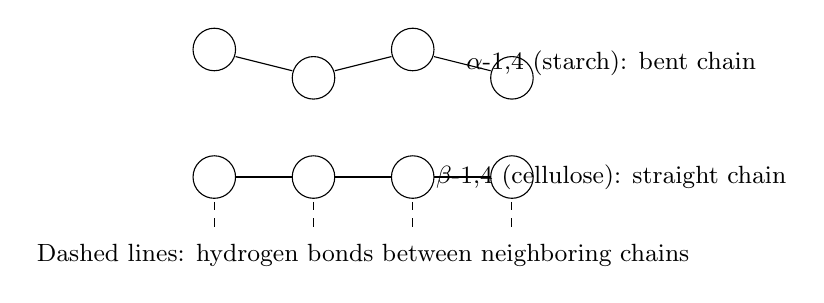
\begin{tikzpicture}[scale=0.9]
\foreach \x/\y in {0/0, 1.4/-0.4, 2.8/0, 4.2/-0.4} \draw (\x,\y) circle (0.3);
\draw (0.3,-0.1) -- (1.1,-0.3); \draw (1.7,-0.3) -- (2.5,-0.1);
\draw (3.1,-0.1) -- (3.9,-0.3);
\node at (5.6,-0.2) {\small $\alpha$-1,4 (starch): bent chain};
\foreach \x in {0, 1.4, 2.8, 4.2} \draw (\x,-1.8) circle (0.3);
\draw (0.3,-1.8) -- (1.1,-1.8); \draw (1.7,-1.8) -- (2.5,-1.8); \draw (3.1,-1.8) -- (3.9,-1.8);
\draw[dashed] (0,-2.15) -- (0,-2.6); \draw[dashed] (1.4,-2.15) -- (1.4,-2.6);
\draw[dashed] (2.8,-2.15) -- (2.8,-2.6); \draw[dashed] (4.2,-2.15) -- (4.2,-2.6);
\node at (5.6,-1.8) {\small $\beta$-1,4 (cellulose): straight chain};
\node at (2.1,-2.9) {\small Dashed lines: hydrogen bonds between neighboring chains};
\end{tikzpicture}
\end{center}

The circles represent glucose rings and the connecting lines glycosidic bonds---again, a human-made representation. Identical building blocks, with only different spatial joint angles, become either food for your mouth or material against the wind. \textbf{Structure determines properties}: the principle repeated since Chapter 3 could hardly be demonstrated more clearly than by carbohydrates.

\section{Glycosidic Bonds: Energy and Rate}

How do you undo a glycosidic bond? Reverse the process: add water back, break the bond, and restore hydroxyls to both ends. This is \textbf{hydrolysis}. Your first step in obtaining energy from rice is hydrolyzing starch into maltose, then into glucose.

Hydrolysis is energetically ``downhill'': breaking polysaccharides into smaller pieces lowers the system's total energy (Chapter 27). Yet a bowl of starch soup left on a table will not turn sweet by itself in a year, nor will paper soaking in water become sugar water in ten years. Energetically allowed, but practically motionless. Why? Chapter 28's rate rule: breaking a glycosidic bond first requires crossing an activation-energy hill, which very few molecules can climb at room temperature.

For rapid breakdown, a catalyst must lower the hill. Salivary amylase is such a catalyst---the secret of rice becoming sweet as you chew. In minutes, the enzyme hydrolyzes starch to maltose, revealing sweetness. Chapter 49 will examine enzymes closely. For now, remember two points: an enzyme changes the reaction pathway and lowers activation energy, but supplies no energy and does not change how far the reaction can ultimately go; and enzymes are particular about joints. Amylase recognizes only $\alpha$ joints and cannot tackle cellulose's $\beta$ joints.

This is the real reason ``humans cannot digest cellulose'': not that cellulose is ``poisonous'' or ``too hard,'' but that our bodies lack the key to its $\beta$ joints. Cows and sheep lack it too. They rely on microorganisms living in their rumens, whose enzymes can break $\beta$ joints. A cow turning grass into flesh is fundamentally a matter of microbes eating grass first and the cow sharing their work's proceeds. Wood-eating termites use the same strategy.

\begin{qiaoliang}
Count the glucose throughout your body. Normal fasting blood glucose is about \ud{1}{g} per liter of blood (medicine reports millimoles per liter, with fasting values around $3.9$--$6.1\ \mathrm{mmol/L}$, converting to roughly 1 gram per liter). An adult has about 5 liters of blood. Multiply:

\[1\ \mathrm{g/L}\times 5\ \mathrm{L}=5\ \mathrm{g}\]

All the glucose in your blood totals only about 5 grams---one teaspoon. How much energy would completely burning those 5 grams release? Complete glucose oxidation releases about \ud{2870}{kJ} per mole (180 grams), so:

\[\frac{5}{180}\times 2870\approx 80\ \mathrm{kJ}\]

Yet even a quietly sitting person's daily basal metabolism requires about \ud{7000}{kJ}: those 80 kJ of blood glucose would last little more than ten minutes. The conclusion is clear: this small stock must be replenished as it is used (by liver glycogen releasing supplies), yet must not grow too large (high blood glucose causes the problems discussed later). Who precisely maintains this ``one-teaspoon'' balance? Later chapters will explain regulation by insulin and other hormones.
\end{qiaoliang}

\section{Now, the Symbols}

Having waited this long, we can let the symbols appear. Glucose's molecular formula is:

\[\chem{C_6H_{12}O_6}\]

Notice that it reports only ``composition,'' not structure. Fructose and galactose have exactly the same composition, also \chem{C_6H_{12}O_6}. A molecular formula does not reveal hydroxyl orientation. That is why this chapter has devoted so much space to rings and joints: the chemical formula is a compressed archive; structure is the full text.

Sucrose hydrolysis:

\[\chem{C_{12}H_{22}O_{11}} + \chem{H_2O} \rightarrow \chem{C_6H_{12}O_6} + \chem{C_6H_{12}O_6}\]

Sucrose is on the left; of the two \chem{C_6H_{12}O_6} molecules on the right, one is glucose and the other fructose. They are isomers, indistinguishable by molecular formula---precisely the symbols' limitation.

Starch hydrolysis (using $n$ for its thousands or tens of thousands of glucose units):

\[(\chem{C_6H_{10}O_5})_n + n\chem{H_2O} \rightarrow n\chem{C_6H_{12}O_6}\]

Notice that starch's ``unit formula'' has one less \chem{H_2O} than glucose: every glucose joined paid a water-molecule fee, so the accounts balance perfectly.

When glucose is finally burned as fuel---called cellular respiration inside cells (discussed from Chapter 52 onward), or combustion in a fire---the net balance is the same:

\[\chem{C_6H_{12}O_6} + 6\chem{O_2} \rightarrow 6\chem{CO_2} + 6\chem{H_2O}\]

Its energy release must be explained by Chapter 27's rule: not ``energy hidden inside sugar molecules,'' but more energy released by forming \chem{C=O} and \chem{O-H} bonds than absorbed by breaking old bonds. Breaking absorbs, forming releases, and the net balance is positive. Precisely because releasing energy does not mean happening unaided (Chapter 28), sugar sits quietly in air until fire or cellular enzyme machinery gets it started.

\begin{shiyan}
\textbf{Experiment One: Chew Out the Sweetness.} Materials: a small spoonful of cooked white rice (or a small piece of plain, unsweetened steamed wheat bread). Procedure: put it in your mouth, resist swallowing, and chew slowly for a full minute, noticing the changing taste near the back of your tongue. What to observe: when does sweetness begin? This is salivary amylase hydrolyzing starch to maltose. Think about why the sweetness does not appear immediately.

\textbf{Experiment Two: Color with Povidone-Iodine.} Materials: pharmacy-bought povidone-iodine (skin antiseptic), a spoonful of rice or a slice of potato, a sugar cube, a small piece of white paper, and a few drops of clean water. Procedure: place one drop of povidone-iodine on each of the rice, sugar cube, and paper, then wait half a minute to inspect the colors. What to observe: rice and potato turn blue-black. Iodine enters the starch helix's channel and forms a dark complex with it. The sugar cube hardly changes; white paper may turn slightly blue because many papers have starch added as sizing during production---a discovery in itself. Comparing color depths even lets you make a semiquantitative guess about which material contains more starch.

Safety note: povidone-iodine is for external use only; keep it out of your mouth and eyes, and remember that it stains clothing. Do not eat any food treated with it. Do not heat it or substitute other chemicals to ``upgrade'' the color test.
\end{shiyan}

\section{Carbohydrates' Three Jobs in the Body}

Now we can inventory their roles. In life's chemical system (Chapter 45), carbohydrates hold at least three jobs.

\textbf{Job One: Fuel.} The ``teaspoon'' of blood glucose is ready-to-use pocket money, on which the brain particularly depends. When pocket money runs low, the body opens its stores: several hundred grams of glycogen in liver and muscle. Why build a densely branching ``bush'' for storage? Because glycogen-breaking enzymes can work only from the ends of side branches. More branches mean more ends and more ``unloading ports'' operating simultaneously. When energy is needed quickly, dozens or hundreds of ends release supplies together. We will calculate the mathematics of this design in the closing challenge. Chapter 52 explains how the energy from glucose breakdown is collected step by step in the ``change jar.''

\textbf{Job Two: Materials.} Plants join glucose into cellulose for their cell walls, supporting all greenery from weeds to tall trees. Cotton is about nine-tenths cellulose; hemp, wood, and paper are cellulose materials too. Shrimp and crab shells and mushroom cell walls use chitin, whose monomer is a ``nitrogen-modified version'' of glucose, likewise joined into long chains by glycosidic bonds. Even the slippery lubricant in your joints and the gel filling your skin consist mainly of negatively charged long-chain carbohydrates. \textbf{Carbohydrates are the biological world's most abundant construction materials}: Earth produces hundreds of billions of tonnes of new cellulose each year, making it the largest contributor among organic substances.

\textbf{Job Three: Identity Tags.} This is the most easily overlooked yet most intricate role. Many short sugar chains hang from every cell's surface, some attached to proteins and others to lipids, like name badges for other cells, antibodies, and viruses to ``read.'' Your blood type is a sugar badge: a sugar chain on red blood cells differs by one terminal sugar to distinguish A, B, and O. Type A adds N-acetylgalactosamine at the end, type B adds galactose, and type O adds nothing. The presence or absence of one sugar molecule marks the immune system's boundary between ``one of us'' and ``intruder.'' Give type B blood to a type A person, and their antibodies attack the foreign red cells as enemies. This is the molecular reason blood types must be checked for transfusion. Strictly speaking, ``blood type'' is thus ``sugar type.'' Cells recognize one another through sugar chains, sperm and eggs match through them, and influenza viruses recognize particular surface sugar chains to locate an entry point. These stories will continue in Chapter 51 on cell membranes.

\section{When Carbohydrates Malfunction: Lactose, Blood Glucose, and Glycation}

\textbf{Translator safety note:} Lactose intolerance and milk allergy are different conditions; do not try the suggested milk/yogurt strategy if milk allergy is possible without professional advice. HbA1c can also be misleading when red-cell lifespan or other conditions affect it. These examples cannot diagnose an individual. See \href{https://www.niddk.nih.gov/health-information/digestive-diseases/lactose-intolerance/eating-diet-nutrition}{NIDDK dietary guidance} and \href{https://www.niddk.nih.gov/health-information/diagnostic-tests/a1c-test}{NIDDK HbA1c guidance}.

The three jobs correspond to three common everyday problems, useful tests of this chapter's model.

\textbf{Lactose intolerance.} Milk's lactose is a disaccharide with a $\beta$ joint, broken by lactase in the small intestine. Almost all infants have ample lactase---otherwise they could not grow on milk---but after weaning, many people's lactase activity naturally declines, especially commonly in East Asian populations. Undigested lactose travels to the large intestine and becomes a feast for gut bacteria. They ferment it, producing gas and acids, causing bloating, rumbling, and diarrhea. Notice two things. First, this is a difference in enzyme abundance, not ``milk allergy,'' which involves the immune system and a different mechanism. Second, dose matters: less enzyme does not mean none. Small, repeated milk servings or switching to yogurt (whose lactic-acid bacteria have already broken down much of the lactose) cause no trouble for many people. Evolutionarily, retaining lactase into adulthood is actually the ``new variation'' in some populations---a story returning in Chapter 83.

\textbf{Blood glucose.} As calculated earlier, blood glucose totals only a teaspoon, and either too much or too little causes problems. Hormones maintain it within a narrow window, with insulin responsible for ``storing food'': making cells absorb glucose and join the excess into glycogen. When this regulation fails---through insufficient insulin or cells responding sluggishly to its signals---persistently high blood glucose is diabetes. This is a medical matter: diagnosis and treatment belong to clinicians and testing standards. Here we only explain the molecular background.

\textbf{Glycation.} Remember that fewer than one in a thousand glucose molecules in water are ``open-chain''? Their reactive terminal aldehydes spontaneously attach to amino groups on proteins and slowly undergo a series of reactions---without enzymes, purely through chemistry. The caramel-colored crust of baking bread and the browning of seared meat are fast, high-temperature versions of the same reaction family, called the Maillard reaction by cooks. At body temperature, it is far slower but never stops: throughout its lifetime, hemoglobin inside a red blood cell is gradually ``glycated'' by glucose. The proportion of glycated hemoglobin (HbA1c) therefore faithfully records the average blood glucose to which the cells have been exposed over roughly three months. Doctors use it to assess long-term glucose control, much more accurately than a single finger-prick reading. Persistent high blood glucose accelerates glycation and produces substances called ``advanced glycation end products'' (AGEs), associated with chronic damage to blood vessels, eyes, and kidneys---one mechanism of diabetic complications.

But evidence requires the complete account: at normal blood glucose, glycation is a slow physiological process occurring in everyone, and the body has cleanup mechanisms. Evidence is weak for commercial ``anti-glycation'' products that turn ``high-glucose pathology'' into ``one bite of sugar ruins your face.'' Sugar is not poison---it is your main fuel. The issues are dose, metabolic condition, and individual differences. This book prescribes no one's diet, but offers a yardstick: whenever a ``molecular mechanism'' is spliced directly into ``consumer scare tactics,'' ask where the evidence is.

\begin{zhengju}
By the late nineteenth century, chemists knew that glucose was \chem{C_6H_{12}O_6}, contained six carbons, and reduced ammoniacal silver solution. But nobody knew its hydroxyl orientations on the four chiral carbons---which of the 16 arrangements it actually had. X-ray crystallography had not even been invented (it arrived in 1912), and no instrument could ``see'' a molecule's three-dimensional structure.

German chemist Emil Fischer used pure chemical logic: modify molecules and examine the products' symmetry. His key move was to oxidize both ends of glucose---the aldehyde and terminal hydroxyl---into carboxyl groups using nitric acid. If an arrangement made the modified molecule symmetrical, it lost optical activity; an asymmetrical one retained it. He combined this with ``upgrading'' reactions that lengthened the sugar chain by one unit and ``downgrading'' reactions that shortened it, tracking the presence and direction of optical rotation in each product. He eliminated possibilities one by one, like checking the alibis of 16 suspects. By 1891, he had established glucose's relative configuration: the one arrangement consistent with all experiments. In 1902, he received the Nobel Prize in Chemistry.

Yet Fischer admitted one thing he could not determine: he had established the relative relationships among carbons, but no experiment then could distinguish whether the entire real structure was the one he drew or its mirror image. He had to ``bet,'' designating one as the standard (the origin of D/L notation), while clearly stating that this was a convention. His chance of guessing correctly? One-half.

Sixty years later, in 1951, Dutch crystallographer Bijvoet used X-ray ``anomalous scattering'' to measure a molecule's absolute configuration for the first time, studying a tartrate salt. The conclusion: Fischer had guessed correctly. The entire stereochemical system of D sugars now had an anchor.

Remember three lessons. First, invisible things can be inferred by elimination, provided each piece of evidence rules out possibilities. Second, scientists may ``bet,'' but must mark what is a bet and what is evidence. Third, a bet may require patience: Fischer did not live to see the verdict, but his reasoning still entered textbooks. We can also answer the earlier question: why does life use almost exclusively D sugars? Once the first enzymes happened to fit D-sugar shapes, the whole metabolic network became ``locked in''; changing hands would require rebuilding all the enzymes. Why that first ``accident'' favored this side, or whether it was purely random, remains honestly unknown---an open puzzle in origin-of-life research.
\end{zhengju}

\section{Where This Carbohydrate Map Falls Short}

The model is useful, but four boundaries need clarification.

\begin{itemize}[itemsep=2pt]
\item \textbf{Six-membered rings are not flat.} A Haworth projection uses a neat hexagon for convenience. The real ring folds into a ``chair'' (Chapter 36 showed cyclohexane's chair), with hydroxyls in ``lying-down'' or ``upright'' positions that differ substantially in stability. The predominance of $\beta$ glucose in water is linked to all its hydroxyls occupying the ``lying-down'' positions.
\item \textbf{A tiny minority need not be unimportant.} Fewer than one in a thousand glucose molecules are open chains, yet glycation, mutarotation, and reactions with many reagents depend on them. Rings and chains continually interconvert in water: when a reaction ``withdraws'' some chains, equilibrium replenishes them. Chapter 31's equilibrium-shift principle quietly operates here.
\item \textbf{This chapter covers only the glucose family.} Nature has hundreds or thousands of monosaccharides. Sugar chains can branch and acquire sulfate or acetyl groups, producing a ``sugar-chain language'' as complex as those of proteins and nucleic acids. Blood types are only its introductory vocabulary.
\item \textbf{Blood glucose is a statistical window, not a verdict.} A single reading changes with meals, exercise, and stress, and individuals differ. The book's numbers explain mechanisms, not self-diagnosis, which requires repeated measurements and medical standards.
\end{itemize}

\begin{wuqu}
``All carbohydrates are sweet, and everything sweet is sugar.'' Both directions are wrong.

First, ``all carbohydrates are sweet'': starch and cellulose are genuine carbohydrates (polysaccharides) without any sweetness. Sweetness requires a small molecule of suitable shape to fit the tongue's sweet receptors; a macromolecule of thousands of linked glucose units cannot fit.

Next, ``everything sweet is sugar'': aspartame is a dipeptide of two amino acids, about 200 times as sweet as sucrose, with a molecular skeleton unrelated to carbohydrates. Saccharin and sucralose are the same in this respect: their shapes merely happen to fool sweet receptors. There is also a bitter historical counterexample: ancient Romans boiled grape juice in lead vessels to make a sweet syrup for flavoring wine. Its sweetness came from lead acetate, commonly called ``sugar of lead,'' which is highly poisonous. Sweet, but neither sugar nor safe.

Sweetness is a matter of tongue receptors; being a carbohydrate is a matter of molecular structure; safety is a matter of dose and toxicology. Three questions, three criteria: none can replace another.
\end{wuqu}

\section{Back to the Opening Four}

Now we can check the answers.

Sugar cube: sucrose, a disaccharide joining glucose and fructose. Its hydroxyls let it dissolve; high-temperature decomposition and rearrangement produce hundreds of new molecules and turn it brown. Caramel aroma is a small chemical storm.

White rice: starch, a helical spring with $\alpha$-1,4 joints. Your amylase recognizes those joints, so chewing brings sweetness; povidone-iodine turns it blue-black because iodine enters the helix's channel.

Tissue: cellulose, long straight chains with $\beta$-1,4 joints, bundled into fibers by interchain hydrogen bonds. Your body lacks the key to this lock, making paper a material rather than food, even though it uses the same building blocks as rice.

Blood type: sugar chains on red blood cells, distinguished as A, B, or O by one terminal sugar. The blood-typing strip recognizes not ``blood,'' but the shape of the sugar-chain end.

Four things, one building block. The difference lies not in the bricks but in the blueprint: joint orientations, chain shapes, and the surfaces from which they hang.

\section{Carbohydrates' Next Stop}

First, add an industrial and ecological account. Cellulose is Earth's most abundantly produced organic substance, used to make paper, cloth, and buildings. Ferment starch and sugars into ethanol, and they also become fuel: many Brazilian cars burn sugarcane ethanol. Nature's largest ``cellulose recycling crews'' are fungi and the microbes in termite guts. Without their breakdown of $\beta$ joints, carbon would pile up in dead branches and leaves. The production end---how plants use sunlight to assemble glucose from carbon dioxide and water---awaits photosynthesis in Chapter 54, with one essential sentence: oxygen comes from water, not carbon dioxide.

Now for a hook. We calculated only 5 grams of blood glucose, yet tens of trillions of cells continually withdraw it as fuel. Cells dare not ``ignite'' glucose: combustion's heat would destroy them. How do they safely extract its 2870 kJ? By dividing sugar breakdown into ten steps, collecting a small payment at each and storing it as molecular change called ATP. This production line is glycolysis, coming in Chapter 52. Before that, the next chapter examines another fuel family---lipids---and why a kilogram stores more than twice as much energy as carbohydrates.

\begin{tiaozhan}
Why does glycogen grow into a ``bush'' rather than a ``long rope''? (Skipping this does not affect the main thread.) Calculate a parallel-processing balance: glycogen-breaking enzymes work inward, one unit at a time, from branch ends. Suppose a glycogen particle stores about 50,000 glucose units. As one unbranched rope, it would have only one working end and release at most $v$ glucose units per unit time. If branching creates 100 ends, the simultaneous release rate becomes $100v$. The cost of branching: each new branch pays an extra water-molecule fee for its $\alpha$-1,6 joint and needs another specialized enzyme to ``prune'' branch points. Liver glycogen must quickly stabilize blood glucose when you are hungry, so it branches densely. Plant starch stores supplies for a whole season and is in less of a hurry, so it branches sparsely. The same chemical bond, assembled differently, becomes either a checking account or a term deposit. Take it further: what if branching is too dense? The ends crowd together so tightly that enzymes cannot enter, preventing breakdown. Real glycogen's branch density sits at the compromise between ``many ends'' and ``not overcrowded.''
\end{tiaozhan}

\section*{Exercises}

\begin{sikaoti}
\item Draw a particle diagram: use hexagons for glucose rings, with a ``flag'' on carbon 1 for its hydroxyl (down for $\alpha$, up for $\beta$). Draw two glucoses joined by $\alpha$-1,4 and by $\beta$-1,4 bonds, label each glycosidic bond, and explain in one sentence why salivary amylase can break only the former. Note beside the diagram that it is a human-made representation.
\item Draw a material-flow diagram for rice from mouth to storage: starch $\rightarrow$ maltose $\rightarrow$ glucose $\rightarrow$ blood $\rightarrow$ liver glycogen. Label each arrow: is the step hydrolysis or condensation? What catalyzes it? Does water enter or leave?
\item Calculate an energy balance: a 500-milliliter bottle of cola contains about \ud{53}{g} of sugar (treated as glucose). If the body completely oxidizes it, how many kilojoules are released? What fraction of a daily basal metabolism of \ud{7000}{kJ} is that? (Glucose's molar mass is \ud{180}{g\cdot mol^{-1}}, and oxidation releases about \ud{2870}{kJ\cdot mol^{-1}}.)
\item Use ``keys and joints'' to explain why lactose-intolerant people readily develop bloating after milk, but often not after yogurt. Why call this a ``normal genetic difference'' rather than a ``disease''? Suggest a feasible milk-drinking strategy in terms of dose.
\item Draw an information-flow diagram: a terminal sugar on a red-cell sugar chain (information) $\rightarrow$ antibody recognition (reading) $\rightarrow$ agglutination (consequence). Explain why type O blood can be given to a type A person (in small amounts in an emergency), whereas the reverse is dangerous. Which molecule carries the information difference?

\textbf{Translator safety note:} This exercise omits essential clinical distinctions: red cells, plasma, and whole blood have different compatibility requirements, and Rh and other antigens matter. Type O is not a blanket permission to transfuse. Only qualified clinicians select and administer blood products with appropriate testing. See \href{https://www.hematology.org/education/patients/blood-basics/blood-safety-and-matching}{American Society of Hematology guidance}.
\item Design a controlled experiment using only povidone-iodine, clean water, and kitchen materials to test whether a particular biscuit contains starch. Describe your experimental group, at least two controls (one known to contain starch and one known not to), a possible false-positive interference (hint: the sizing in the paper experiment), and a way to rule it out.
\end{sikaoti}
